\def\disciplina {Calculo A}
\def\turma {00000}
\def\semestre {2016.1}
\def\numerodealunos {63}
\documentclass{article}
\usepackage[utf8]{inputenc}
\usepackage[T1]{fontenc}
\usepackage{graphicx}
\usepackage{palatino}
\usepackage{subcaption}
\usepackage{ctable}
\title{Relatório de Notas de \disciplina\\Semestre \semestre}
\author{Melissa Weber Mendonça}
\date{}
\begin{document}
\maketitle
\section*{Distribuição de Notas}

Abaixo, a Tabela~\ref{tab:tudo} contendo as notas de \disciplina\ dos alunos da Turma \turma\ no semestre de \semestre.

\begin{table}[h!]
   \begin{center}
      %    # Escrever tabela com os dados completos no arquivo
    with open('tabelacompleta.tex', 'w') as f:
        print>>f, "\\begin{tabular}{l c c c c} \\toprule"
        print>>f, " & ".join(df.columns)+u" & Média Final\\\\\\midrule"
        for i in range(0,numalunos):
            linha = " & ".join(np.array2string(df.values[i,:]).strip("[","]"))+mediasfinais[i]+"\\"
        
        print >>f, "\\end{tabular}"


\begin{tabular}{l c c c c} \toprule
Prova 1 & Prova 2 & Prova 3 & Média Final\\\midrule

      \caption{Tabela representando os dados completos.}
      \label{tab:tudo}
   \end{center}
\end{table}

As Figuras~\ref{fig:prova1}, \ref{fig:prova2} e \ref{fig:prova3} representam a distribuição das notas para os \numerodealunos\ alunos desta turma.

\begin{figure}[ht]
   \centering
   \begin{subfigure}[b]{0.3\textwidth}
      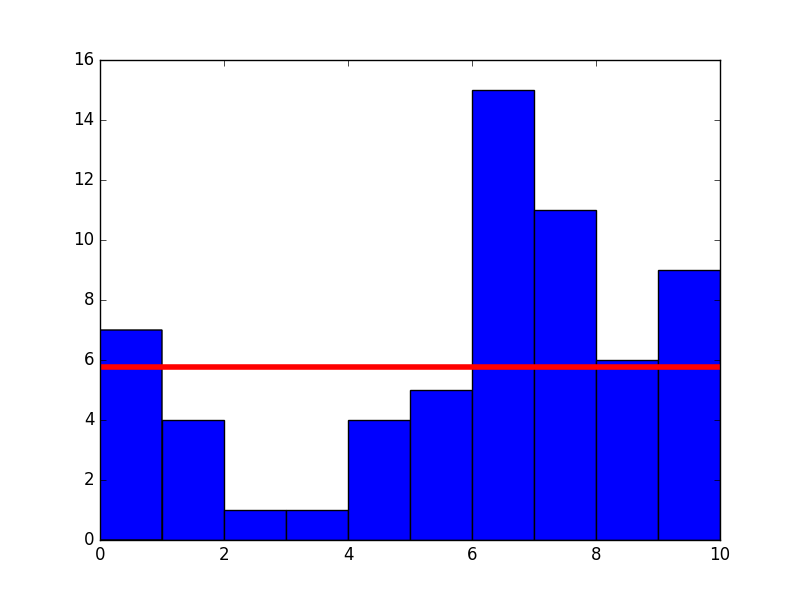
\includegraphics[width=4cm]{prova1.png}
      \caption{Notas da Prova 1.}
      \label{fig:prova1}
   \end{subfigure}
   ~
   \begin{subfigure}[b]{0.3\textwidth}
      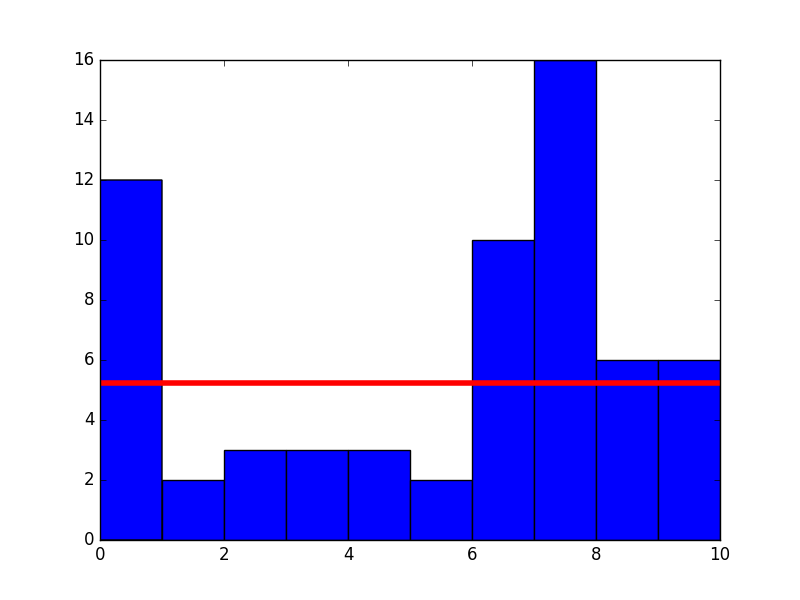
\includegraphics[width=4cm]{prova2.png}
      \caption{Notas da Prova 2.}
      \label{fig:prova2}
   \end{subfigure}
   ~
   \begin{subfigure}[b]{0.3\textwidth}
      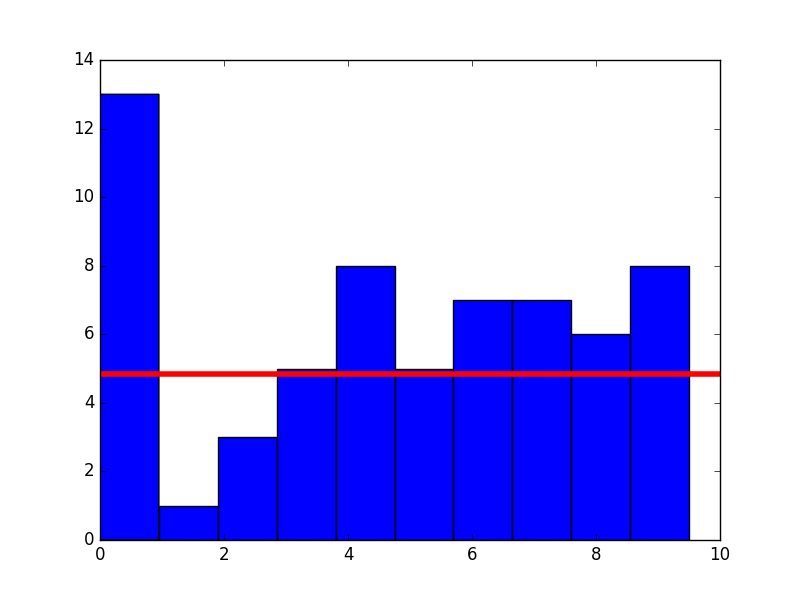
\includegraphics[width=4cm]{prova3.png}
      \caption{Notas da Prova 3.}
      \label{fig:prova3}
   \end{subfigure}
   \caption{Distrubuição de notas nas 3 provas.}
\end{figure}

\subsection*{Aprovados vs. Reprovados}

As Figuras~\ref{fig:aprovados} e \ref{fig:reprovados} mostram as notas dos alunos que terminaram aprovados e reprovados no curso, respectivamente.

\begin{center}
\begin{figure}[ht]
   \centering
   \begin{subfigure}[h]{0.45\textwidth}
      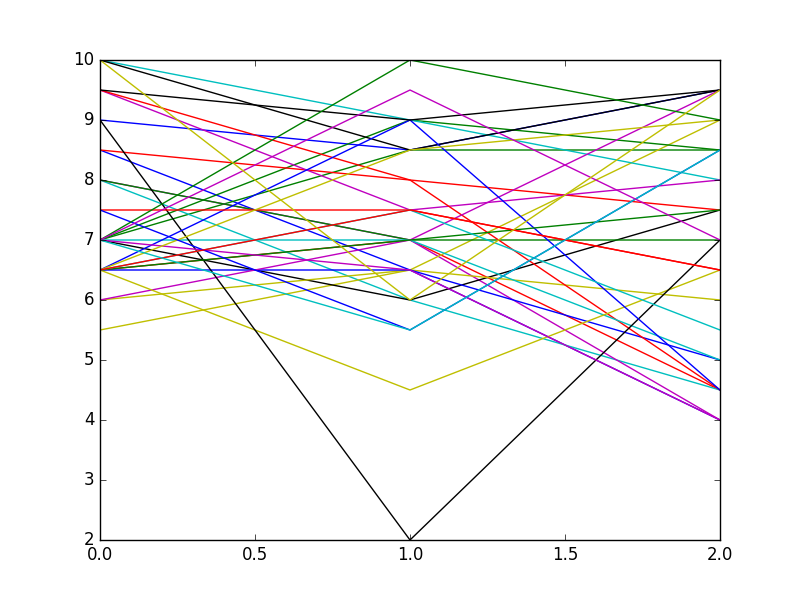
\includegraphics[width=4cm]{notasaprovados.png}
      \caption{Notas das 3 provas dos alunos aprovados.}
      \label{fig:aprovados}
   \end{subfigure}
   ~
   \begin{subfigure}[h]{0.45\textwidth}
      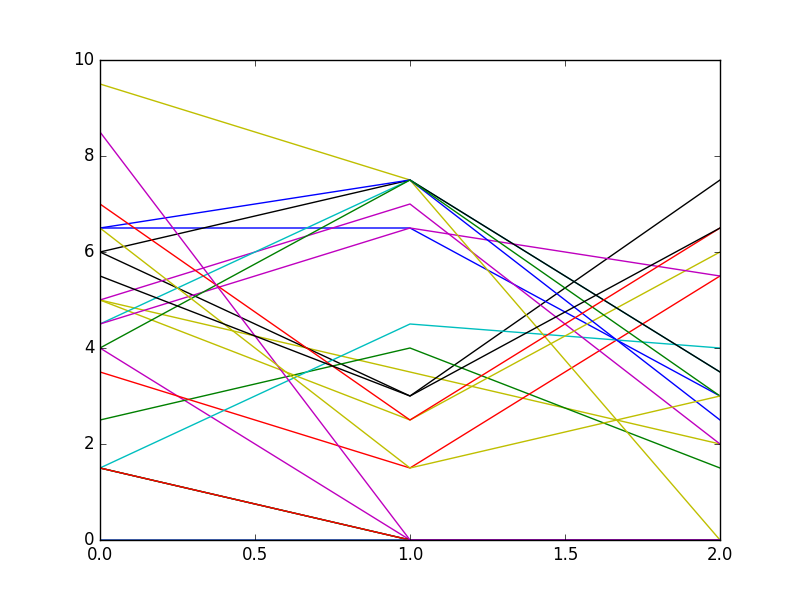
\includegraphics[width=4cm]{notasreprovados.png}
      \caption{Notas das 3 provas dos alunos reprovados.}
      \label{fig:reprovados}
   \end{subfigure}
\end{figure}
\end{center}

\end{document}
